\documentclass[border=10pt]{standalone}
\usepackage[svgnames]{xcolor}
\usepackage{amsmath}
\usepackage{pgfplots}
\pgfplotsset{compat=newest}
\usepackage[sfdefault]{FiraSans}
\usepackage{FiraMono}
\renewcommand*\familydefault{\sfdefault}
\begin{document}
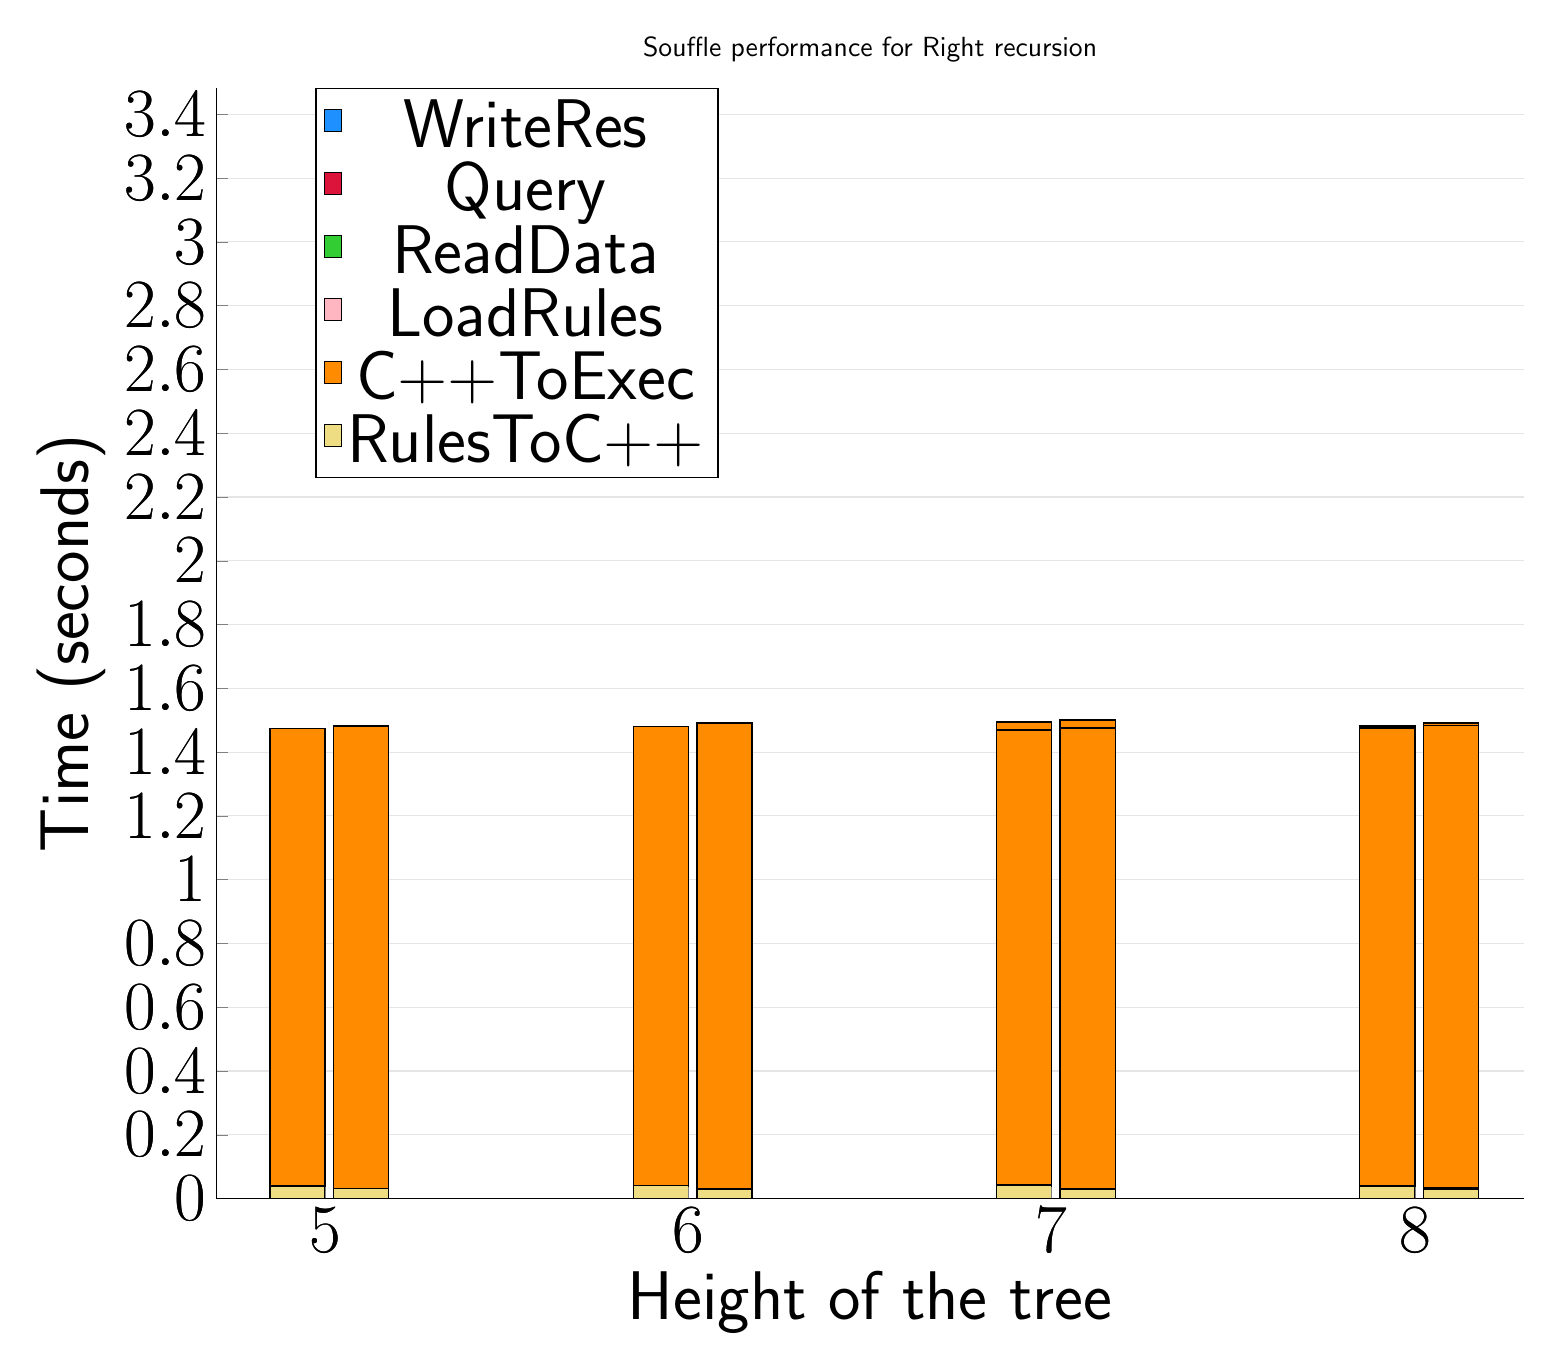
\begin{tikzpicture}
	\begin{axis}[
			ybar stacked,
			title={Souffle performance for Right recursion},
			bar shift=-10pt,
			width=1.5\textwidth,
			bar width=0.7cm,
			ymajorgrids, tick align=inside,
			major grid style={draw=gray!20},
			xtick=data,
			ymin=0, ymax=3.4829999685287474,
			axis x line*=bottom,
			axis y line*=left,
			enlarge x limits=0.1,
			legend style={
					at={(0.23, 1)},
					anchor=north,
					legend columns=1,
					font=\Huge,
				},
			ylabel={Time (seconds)},
			xlabel={Height of the tree},
			label style={font=\Huge},
			tick label style={font=\Huge},
		]
		\addlegendimage{fill=DodgerBlue, draw=black, line width=0.2pt}
		\addlegendentry{WriteRes}
		\addlegendimage{fill=Crimson, draw=black, line width=0.2pt}
		\addlegendentry{Query}
		\addlegendimage{fill=LimeGreen, draw=black, line width=0.2pt}
		\addlegendentry{ReadData}
		\addlegendimage{fill=LightPink, draw=black, line width=0.2pt}
		\addlegendentry{LoadRules}
		\addlegendimage{fill=DarkOrange, draw=black, line width=0.2pt}
		\addlegendentry{C++ToExec}
		\addlegendimage{fill=LightGoldenrod, draw=black, line width=0.2pt}
		\addlegendentry{RulesToC++}
		\addplot +[fill=LightGoldenrod, draw=black, line width=0.5pt] coordinates {
				(5, 0.03900001049041748)
				(6, 0.040999984741210936)
				(7, 0.04100000858306885)
				(7, 0.04199995994567871)
				(7, 0.04100000858306885)
				(8, 0.039999985694885255)
				(8, 0.04100000858306885)
				(8, 0.04100005626678467)
			};
		\addplot +[fill=DarkOrange, draw=black, line width=0.5pt] coordinates {
				(5, 1.4349999904632569)
				(6, 1.4390000343322753)
				(7, 1.4279999494552613)
				(7, 1.4260000705718994)
				(7, 1.4509999752044678)
				(8, 1.4350000143051147)
				(8, 1.4370000123977662)
				(8, 1.4359999656677247)
			};
		\addplot +[fill=LightPink, draw=black, line width=0.5pt] coordinates {
				(5, 0.0)
				(6, 0.0)
				(7, 0.0)
				(7, 3.1545900000000006e-05)
				(7, 0.0)
				(8, 0.0)
				(8, 3.88208e-05)
				(8, 0.0)
			};
		\addplot +[fill=LimeGreen, draw=black, line width=0.5pt] coordinates {
				(5, 0.0004247957)
				(6, 0.0004992085000000001)
				(7, 0.0006365212999999999)
				(7, 0.0006537998000000001)
				(7, 0.0006286000000000001)
				(8, 0.0008918124000000001)
				(8, 0.0010226203)
				(8, 0.0009274871000000001)
			};
		\addplot +[fill=Crimson, draw=black, line width=0.5pt] coordinates {
				(5, 0.0001109501)
				(6, 0.00034189180000000004)
				(7, 0.0008216708)
				(7, 0.0008673338000000001)
				(7, 0.0007870584)
				(8, 0.0019454069999999997)
				(8, 0.0020482169999999997)
				(8, 0.0019350489999999999)
			};
		\addplot +[fill=DodgerBlue, draw=black, line width=0.5pt] coordinates {
				(5, 0.00046331259999999995)
				(6, 0.00045935029999999996)
				(7, 0.0005430627)
				(7, 0.0006160919)
				(7, 0.0004564541)
				(8, 0.0011776631999999999)
				(8, 0.0010787912)
				(8, 0.0010210500000000001)
			};
	\end{axis}
	\begin{axis}[
			ybar stacked,
			bar shift=13pt,
			width=1.5\textwidth,
			bar width=0.7cm,
			ymajorgrids, tick align=inside,
			major grid style={draw=none},
			xtick=data,
			ymin=0, ymax=3.4829999685287474,
			axis x line*=none,
			axis y line*=none,
			enlarge x limits=0.1,
			label style={font=\Huge},
			tick label style={font=\Huge},
		]
		\addplot +[fill=LightGoldenrod, draw=black, line width=0.5pt] coordinates {
				(5, 0.031999999999999994)
				(6, 0.030000000000000006)
				(7, 0.030000000000000006)
				(7, 0.030000000000000006)
				(7, 0.031000000000000007)
				(8, 0.030000000000000006)
				(8, 0.030000000000000006)
				(8, 0.032999999999999995)
			};
		\addplot +[fill=DarkOrange, draw=black, line width=0.5pt] coordinates {
				(5, 1.4499999999999997)
				(6, 1.4600000000000002)
				(7, 1.4449999999999998)
				(7, 1.4479999999999997)
				(7, 1.4689999999999999)
				(8, 1.454)
				(8, 1.459)
				(8, 1.4499999999999997)
			};
		\addplot +[fill=LightPink, draw=black, line width=0.5pt] coordinates {
				(5, 0.0)
				(6, 0.0)
				(7, 0.0)
				(7, 3.12e-05)
				(7, 0.0)
				(8, 0.0)
				(8, 1.01e-05)
				(8, 0.0)
			};
		\addplot +[fill=LimeGreen, draw=black, line width=0.5pt] coordinates {
				(5, 0.0003510000000000001)
				(6, 0.0004326)
				(7, 0.0005727000000000001)
				(7, 0.0005906)
				(7, 0.0005552)
				(8, 0.0008234999999999999)
				(8, 0.0008766000000000002)
				(8, 0.0008435)
			};
		\addplot +[fill=Crimson, draw=black, line width=0.5pt] coordinates {
				(5, 0.00011040000000000001)
				(6, 0.0003412)
				(7, 0.000821)
				(7, 0.0008640999999999999)
				(7, 0.0007863999999999999)
				(8, 0.0019447999999999996)
				(8, 0.0020185)
				(8, 0.0019312999999999997)
			};
		\addplot +[fill=DodgerBlue, draw=black, line width=0.5pt] coordinates {
				(5, 0.0002695)
				(6, 0.00032779999999999994)
				(7, 0.00048110000000000004)
				(7, 0.0005166)
				(7, 0.00045460000000000005)
				(8, 0.0009165)
				(8, 0.000911)
				(8, 0.0009096)
			};
	\end{axis}
\end{tikzpicture}

\end{document}
